\section{Lecture du numéro d'immatriculation}
Pour la lecture des caractères présents sur la plaque détectée, nous avons utilisé l’approche proposé par certains chercheurs de l’UM6P \cite{Alahyane2021OpenDF}. Cette approche consiste à utiliser un modèle pour détecter les caractères et classifier en même temps. Pour l’entraînement du modèle, ils sont appel à l’architecture YOLOv3. La précision obtenue sur les données d’entraînement est de \textbf{94,42\%} et sur les données de test \textbf{82,38\%}. Puisque ces résultats sont satistfaisants, nous avons adopté la même approche mais avec une version plus récente de YOLO: version 4. L'avantage avec cette approche par l'approche classique de l'OCR est que nous n'avons pas vraiment besoin d'une phase de prétraitement de l'image au préalable. Ceci participe donc à la rapidité de l'ensemble de système ANPR. Décrivons maintenant chaque étape suivie pour obtenir notre modèle.
    \subsection{Acquisition des données}
    Cette phase est très important car détermine la qualité du modèle. Une mauvaise qualité de données conduit inéluctablement à une mauvais modèle. Nous avons donc pris soin de collecter une important masse diversifiée d’images de plaques marocaines. Pour y parvenir, nous avons pris les images contenant des véhicules au Maroc utilisées lors de la précédente phase. Grâce à un script Python et avec le modèle de détection de plaques conçu précédemment nous avons extrait les images des plaques. Nous avons donc pu réunir \textbf{3570 images}. A l’aide de l’outil d’annotation LabelImg, nous avons annoté ces images suivant \textbf{16 classes (\textit{0, 1, 2, 4, 5, 6, 7, 8, 9, a, b, waw, d, h, w})}.
    \begin{figure}[H]
        \centering
        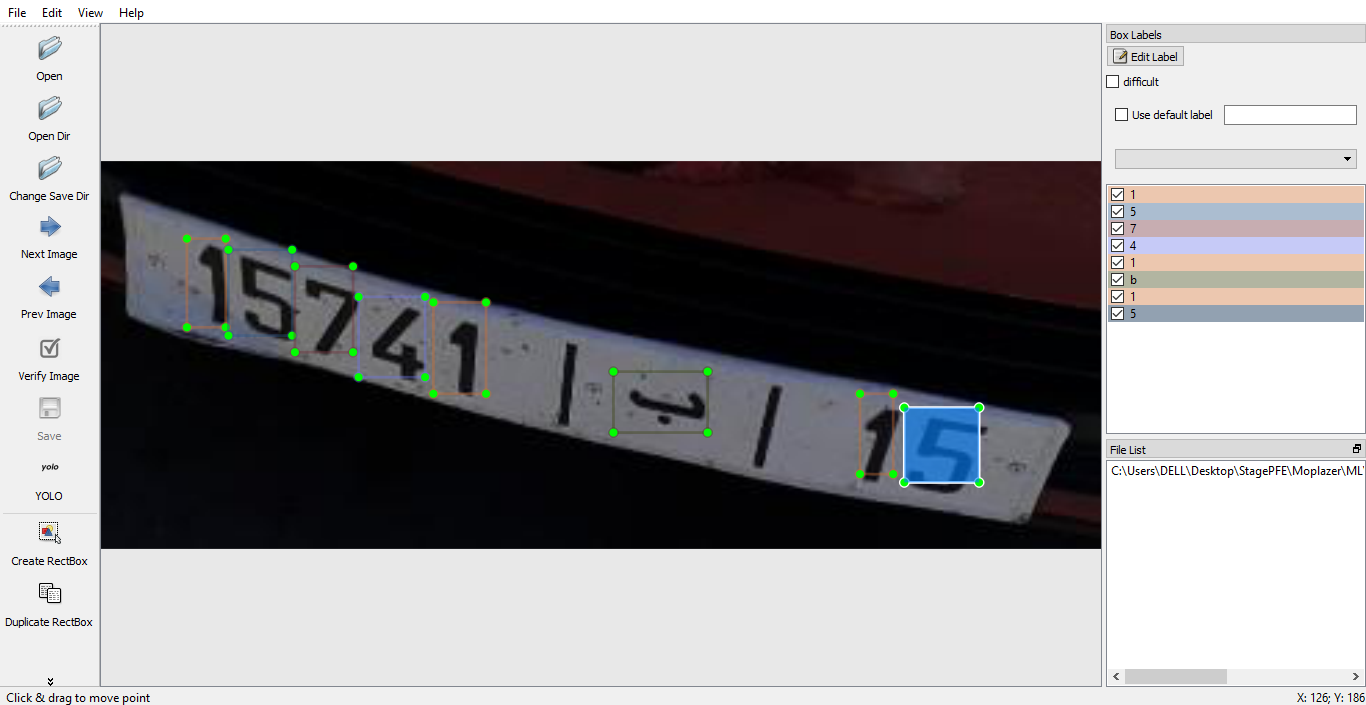
\includegraphics[scale=0.3]{exampleAnnotation}
        \caption{Exemple d'annotation de plaque sur LabelImg}
    \end{figure}
    \subsection{Nettoyage et préparation}
    Pour cette phase, nous avons dans un premier temps effectuer quelques prétraitements sur les images collectées (redimensionnement et auto-orientation). Dans un second, pour augmenter le volume des données, nous avons créé de nouvelles données à partir des 3570 originales. Cette augmentation a été faite sur la plateforme Roboflow en utilisant plusieurs procédés comme la \textbf{saturation}, \textbf{modification de la luminosité}, l’\textbf{ajout des bruits et de flous}. Ces procédés nous ont permis d’avoir au total \textbf{8989 images annotées de plaques marocaines}. Nous avons analysé les proportions de chaque classes dans notre base de 8989 images et le graphe suivant les illustre. 
        \begin{figure}[H]
            \centering
            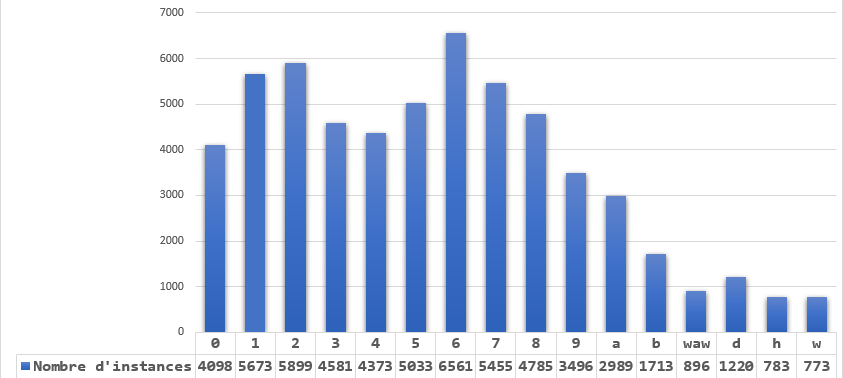
\includegraphics[scale=0.5]{proportionsClasses}
            \caption{Proportions des classes}
        \end{figure}
    \subsection{Entraînement du modèle}
    Avant l’entraînement proprement dit, nous avons subdivisé nos deux données en deux: 90\% pour l’entraînement et 10\% pour le test. Nous avons par la suite effectué l’entraînement sur Google Colab avec les même paramètres que précédemment sauf quelques modifications:
    \begin{itemize}
        \item \textbf{Utilisation du \href{https://github.com/AlexeyAB/darknet/}{repertoire darknet d'AlexeyAB}}
        \item \textbf{Utilisation de fichier de configuration} \href{https://github.com/AlexeyAB/darknet/blob/master/cfg/yolov4-tiny-3l.cfg}{yolov4-tiny\_3l.cfg}: Toutefois nous avons modifié certains paramètres dans ce fichier.
        \begin{table}[H]
            \centering
            \begin{tabular}{|l|c|}
                \hline
                \rowcolor{Gray}
                \textbf{Paramètres} & \textbf{Nouvelle valeur} \\ \hline
                batch & 64 \\ \hline
                subdivisions & 32 \\ \hline
                width & 416 \\ \hline
                height & 416 \\ \hline
                max\_batches & 10000 \\ \hline
                steps & 8000, 9000 \\ \hline
                classes & 16 \\ \hline
                filters (couche de convolution avant couche yolo) & 63 \\ \hline 
            \end{tabular}
            \caption{Quelques paramètres du fichier de configuration YOLO pour le modèle OCR}
        \end{table}
    \end{itemize}
    Le graphe suivant montre l'évolution de la performance du modèle au cours de l'entraînement: la précision maximale atteint par le modèle est de \textbf{95,1\%}.
        \begin{figure}[H]
            \centering
            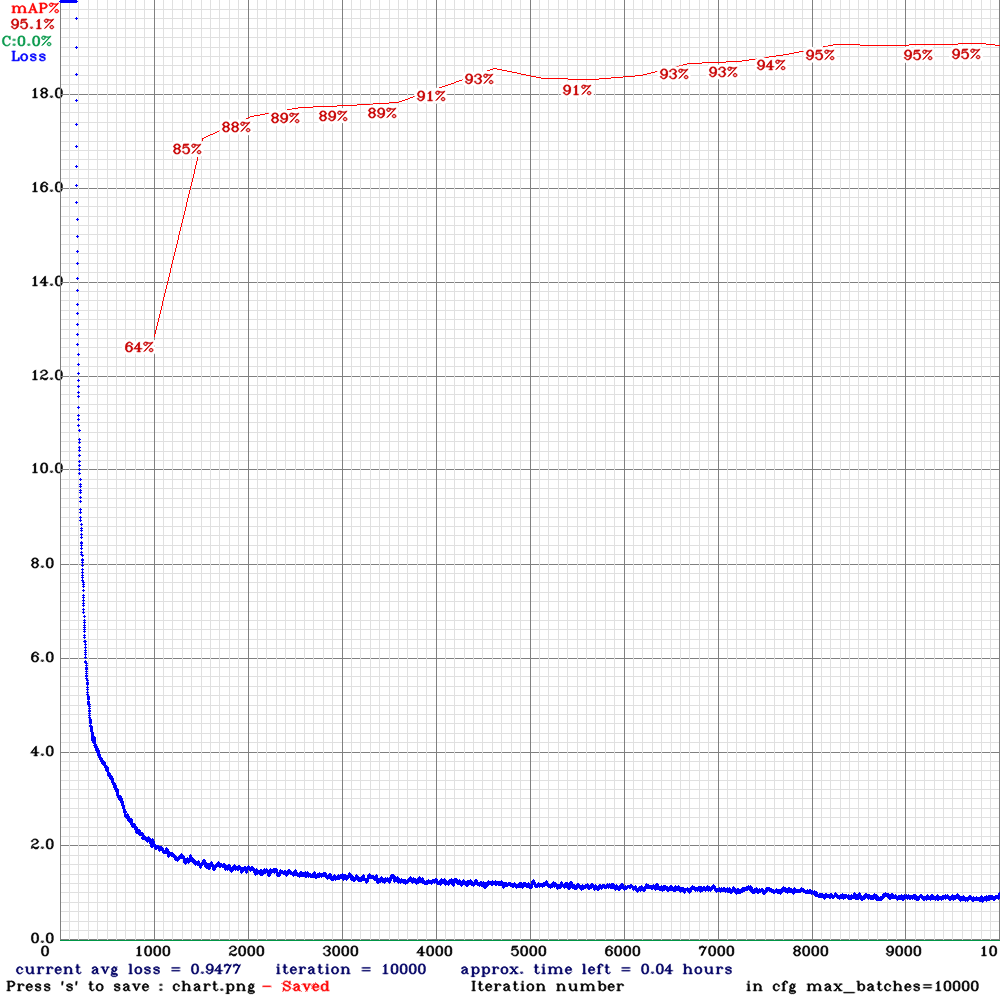
\includegraphics[scale=0.3]{chart2.png}
            \caption{Évolution de la performance du modèle}
        \end{figure}
    \subsection{Résultats et évaluation}
    Pour évaluer notre modèle de lecture du matricule, nous avons collecté des images contenant des véhicules. Dans un premier temps, nous avons utilisé le modèle de détection de plaques pour localiser les plaques sur les images. Dans un second temps, nous avons utilisé le modèle courant pour détecter les caractères sur les plaques. Le tableau suivant les résultats de la performance du modèle.
    \begin{table}[H]
        \centering
        \begin{tabular}{|l|l|}
            \hline
            \rowcolor{Gray}
            \textbf{Evaluation} & \textbf{Valeur} \\ \hline
            Nombre de caractères correctement détectés (VP) & \textbf{302} \\ \hline
            Nombre de caractères non détectés (FN) & \textbf{11} \\ \hline
            Nombre de fausses détections (FP) & \textbf{12} \\ \hline
            Précision & \textbf{96,18\%} \\ \hline
            Rappel & \textbf{96,48\%} \\ \hline
        \end{tabular}
        \caption{Evaluation du modèle de lecture du matricule}
    \end{table}
    Comme pour le modèle de détection de plaques, la précision et le rappel du modèle de lecture des matricules sont très élevés. Ceci nous permet de dire que notre système est globalement très précis. Voic quelques exemples de lecture des plaques d'immatriculation.
    \begin{figure}[H]
        \begin{subfigure}{0.3\textwidth}
            \centering
            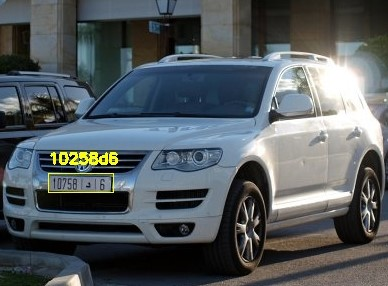
\includegraphics[width=\textwidth]{plateDetect1}
        \end{subfigure}
        \hfill
        \begin{subfigure}{0.3\textwidth}
            \centering
            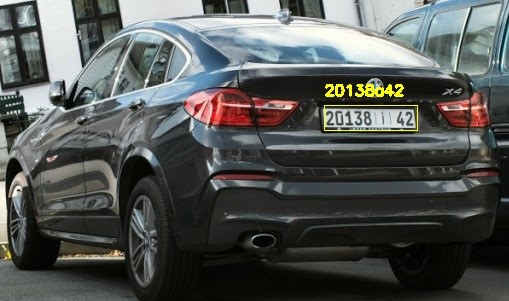
\includegraphics[width=\textwidth]{plateDetect2}
        \end{subfigure}
        \hfill
        \begin{subfigure}{0.3\textwidth}
            \centering
            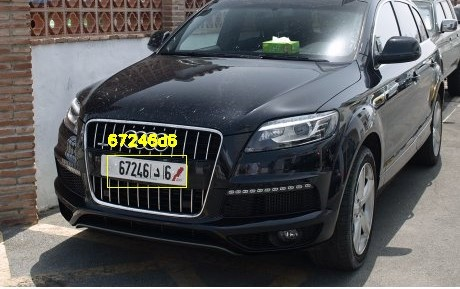
\includegraphics[width=\textwidth]{plateDetect3}
        \end{subfigure}
        \caption{Exemples de lecture des matricules des véhicules}
    \end{figure}
